\documentclass[border=10pt]{standalone}
\usepackage{tikz}
\usetikzlibrary{positioning, calc, arrows.meta}
\usepackage{amsmath, amssymb}

\begin{document}
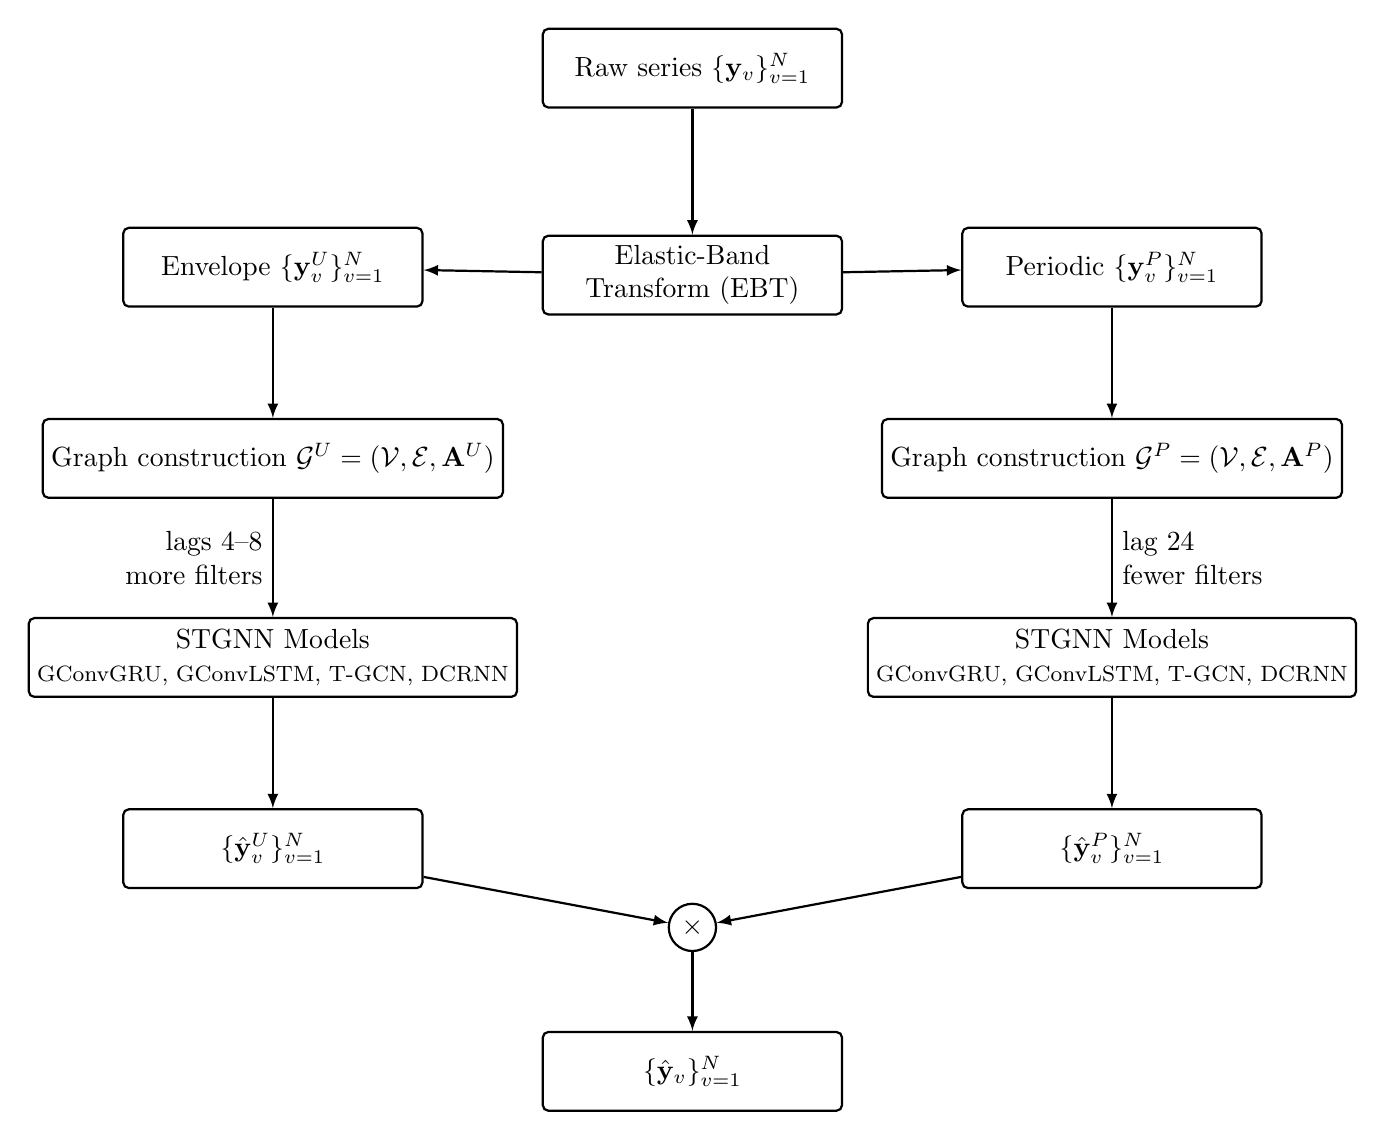
\begin{tikzpicture}[>=latex, thick]
\tikzset{
  blk/.style={draw, rounded corners=2pt, align=center, inner sep=3pt, minimum width=38mm, minimum height=10mm},
  op/.style ={draw, circle, inner sep=1pt, minimum size=6mm}
}

% row 1
\node[blk] (y) {Raw series $\{\mathbf{y}_v\}_{v=1}^{N}$};

% row 2
\node[blk, below=16mm of y] (ebt)  {Elastic-Band\\Transform (EBT)};
\node[blk, below left=15mm and 15mm of y] (yU) {Envelope $\{\mathbf{y}_v^{U}\}_{v=1}^{N}$};
\node[blk, below right=15mm and 15mm of y] (yP) {Periodic $\{\mathbf{y}_v^{P}\}_{v=1}^{N}$};

\draw[->] (y) -- (ebt);
\draw[->] (ebt) -- (yU);
\draw[->] (ebt) -- (yP);

% row 3 : 그래프 구성
\node[blk, below=14mm of yU] (graphU) {Graph construction $\mathcal{G}^{U}=({\cal V},{\cal E},{\mathbf A}^U)$};
\node[blk, below=14mm of yP] (graphP) {Graph construction $\mathcal{G}^{P}=({\cal V},{\cal E},{\mathbf A}^P)$};

\draw[->] (yU) -- (graphU);
\draw[->] (yP) -- (graphP);

% row 4 : STGNN
\node[blk, below=15mm of graphU] (modelU) {STGNN Models\\\footnotesize GConvGRU, GConvLSTM, T-GCN, DCRNN};
\node[blk, below=15mm of graphP] (modelP) {STGNN Models\\\footnotesize GConvGRU, GConvLSTM, T-GCN, DCRNN};

\draw[->] (graphU) -- node[left, align=right]{lags 4--8\\more filters} (modelU);
\draw[->] (graphP) -- node[right, align=left]{lag 24\\fewer filters} (modelP);

% row 5 : predictions
\node[blk, below=14mm of modelU] (predU) {$\{\hat{\mathbf{y}}^{U}_{v}\}_{v=1}^{N}$};
\node[blk, below=14mm of modelP] (predP) {$\{\hat{\mathbf{y}}^{P}_{v}\}_{v=1}^{N}$};

\draw[->] (modelU) -- (predU);
\draw[->] (modelP) -- (predP);

% combine
\node[op] (mul) at ($(predU)!0.5!(predP)-(0,10mm)$) {$\times$};
\draw[->] (predU) -- (mul);
\draw[->] (predP) -- (mul);
\node[blk, below=10mm of mul] (final) {$\{\hat{\mathbf{y}}_{v}\}_{v=1}^{N}$};
\draw[->] (mul) -- (final);

\end{tikzpicture}
\end{document}
